\documentclass[letterpaper, 12pt]{article}
\usepackage{geometry}
\usepackage{pgfplots}

\pgfplotsset{compat=1.13}
\usepgfplotslibrary{fillbetween}
\usetikzlibrary{patterns}
\geometry{letterpaper, margin=1in}

\renewcommand*{\arcsin}{\sin^{-1}}
\renewcommand*{\arccos}{\cos^{-1}}
\renewcommand*{\arctan}{\tan^{-1}}
\newcommand*{\arccot}{\cot^{-1}}
\newcommand*{\arcsec}{\sec^{-1}}
\newcommand*{\arccsc}{\csc^{-1}}
\newcommand*{\diff}{\mathrm{d}}
\newcommand*{\Diff}[1]{\mathrm{d^#1}}
\newcommand*{\e}{\mathrm{e}}

\title{Section 6.1}
\author{Alvin Lin}
\date{Calculus II: August 2016 - December 2016}

\begin{document}

\maketitle

\section*{Problem 3}
\[ x = \e^{y} \quad x = y^{2}-2 \]
\[ a = -1 \quad b = 1 \]
\[ \int_{-1}^{1}{\e^{y}-(y^{2}-2)\diff{y}} \]
\[ \bigg[\e^{y}-\frac{y^{3}}{3}+2y\bigg]_{-1}^{1} \]
\[ [\e-\frac{1}{3}+2]-[\e^{-1}-\frac{-1}{3}-2] \]
\[ = \e-\frac{1}{\e}+\frac{10}{3} \]

\section*{Problem 8}
\[ y = x^{2}-4x \quad y = 2x \]
\[ x^{2}-4x = 2x \]
\[ x^{2}-6x = x(x-6) = 0 \]
\[ x = 0 \quad x = 6 \]
\[ \int_{0}^{6}{2x-(x^{2}-4x)\diff{x}} \]
\[ \bigg[\frac{6x^{2}}{2}-\frac{x^{3}}{3}\bigg]_{0}^{6} \]
\[ [3\times6^{2}-\frac{6^{3}}{3}]-[0-0] \]
\[ 108-72 \]
\[ = 36 \]

\section*{Problem 13}
\[ y = 12-x^{2} \quad y = x^{2}-6 \]
\[ 12-x^{2} = x^{2}-6 \]
\[ 2x^{2}-18 = x^{2}-9 = (x+3)(x-3) = 0 \]
\[ x = -3 \quad x = 3 \]
\[ \int_{-3}^{3}{12-x^{2}-(x^{2}-6)\diff{x}} \]
\[ 2\int_{0}^{3}{18-2x^{2}\diff{x}} = 4\int_{0}^{3}{9-x^{2}\diff{x}} \]
\[ 4\bigg[9x-\frac{x^{3}}{3}\bigg]_{0}^{3} \]
\[ 4\bigg([9(3)-\frac{3^{3}}{3}]-[0-0]\bigg) \]
\[ 4(27-9) \]
\[ = 72 \]

\section*{Problem 16}
\[ y = 2-\cos(x) \quad y = \cos(x) \]
\begin{center}
  \begin{tikzpicture}
    \begin{axis}[axis lines=middle,
                 xlabel=\(x\),
                 ylabel=\(y\),
                 ymin=-2,
                 ymax=4,
                 xtick={0,6},
                 ytick=\empty]
    \addplot[name path=F,
             blue,
             domain={0:6.5}]{2-cos(deg(x))} node[pos=0.5, above]
             {\( f(x)=2-\cos(x) \)};
    \addplot[name path=G,
             green,
             domain={0:6.5}]{cos(deg(x))} node[pos=0.5, below]
             {\( g(x)=\cos(x) \)};
    \addplot[color=brown!30] fill between [
             of=F and G, soft clip third={domain=0:6}];
    \end{axis}
  \end{tikzpicture}
\end{center}
\[ \int_{0}^{2\pi}{2-\cos(x)-(\cos(x))\diff{x}} \]
\[ \bigg[2x-2\sin(x)\bigg]_{0}^{2\pi} \]
\[ \bigg[2(2\pi)-2\sin(2\pi)\bigg]-\bigg[0-2\sin(0)\bigg] \]
\[ = 4\pi \]

\section*{Problem 23}
\[ y = \frac{1}{8}x^{2} \quad y = (2x)^{\frac{1}{3}} \]
\begin{center}
  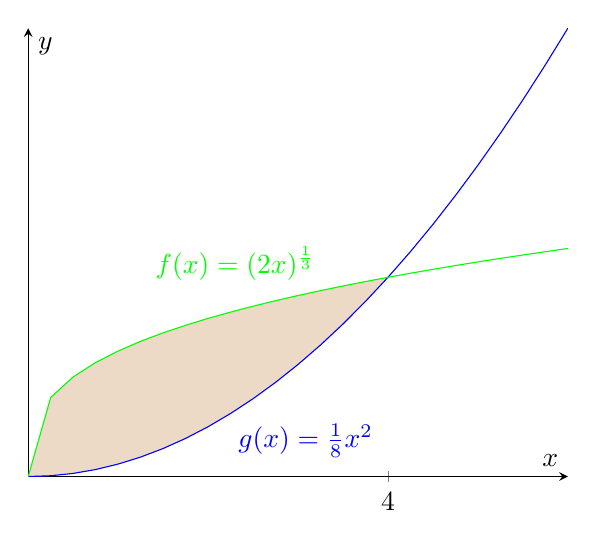
\begin{tikzpicture}
    \begin{axis}[axis lines=middle,
                 xlabel=\(x\),
                 ylabel=\(y\),
                 xtick={0,4},
                 ytick=\empty]
    \addplot[name path=G,
             blue,
             domain={0:6}]{pow(x,2)/8} node[pos=0.3, anchor=north west]
             {\( g(x)=\frac{1}{8}x^{2} \)};
    \addplot[name path=F,
             green,
             domain={0:6}]{pow(2*x, 0.3333)} node[pos=0.6, anchor=south east]
             {\( f(x)=(2x)^{\frac{1}{3}} \)};
    \addplot[color=brown!30] fill between [
             of=F and G, soft clip={domain=0:4}];
    \end{axis}
  \end{tikzpicture}
\end{center}
\[ \int_{0}^{4}{(2x)^{\frac{1}{3}}-\frac{1}{8}x^{2}\diff{x}} \]
\[ \int_{0}^{4}{(2x)^{\frac{1}{3}}\diff{x}}-
   \int_{0}^{4}{\frac{1}{8}x^{2}\diff{x}} \]
\[ Let: u = 2x \]
\[ \diff{u} = 2\diff{x} \]
\[ \frac{1}{2}\int{u^{\frac{1}{3}}\diff{u}}-
   \frac{1}{8}\int_{0}^{4}{x^{2}\diff{x}} \]
\[ \frac{1}{2}\frac{3u^{\frac{4}{3}}}{4}-\frac{1}{8}\frac{x^{3}}{3} \]
\[ \bigg[\frac{3(2x)^{\frac{4}{3}}}{8}-\frac{x^{3}}{24}\bigg]_{0}^{4} \]
\[ [\frac{3(8)^{\frac{4}{3}}}{8}-\frac{4^{3}}{24}]-[0-0] \]
\[ [6-\frac{8}{3}] \]
\[ = \frac{16}{3} \]

\begin{center}
  If any errors are found, please contact me at alvin.lin.dev@gmail.com
\end{center}

\end{document}
